\documentclass{report}
\usepackage{hyperref} 
\usepackage{xcolor, color}
\usepackage{fullpage}
\usepackage{listings}
\usepackage{graphicx}
\usepackage{amsmath}
\usepackage{mathtools}
\usepackage{multirow}
\usepackage{relsize}
\usepackage{fancyhdr}
%\pagestyle{fancy}
\usepackage{multicol}
\usepackage{titlecaps}
\usepackage{titlesec}

\definecolor{medium-blue}{rgb}{0,0,1}
\definecolor{mygray}{rgb}{0.8,0.8,0.8}

\hypersetup{colorlinks, urlcolor={medium-blue}}


\begin{document}

%\vspace{3cm}
%\begin{center}
%\bigskip
%\Large{\today}
%\vspace{0.5cm}

%{\titlecap{Embedded Systems} 
%\vspace{0.3cm}}\\
%\vspace{0.4cm}
%\bigskip
%\rule{\linewidth}{0.5mm}
%\titlecap{Natural logarithm implementation for BFloat16 FPU}\\
%\vspace{0.4cm}
%\titlecap{REV. 0.1}
%\end{center}

%\vfill
%\begin{multicols}{2}
%
\includegraphics[height=3cm]{images/Logo_Polimi}

%\raggedright{\textbf{Authors} (in alphabetical order): {\\
%Andrea Buffoli\\
%Matteo Giacomello\\
%Artem Glukhov\\
%Giacomo Ticchi}\\
%}
%\end{multicols}

%\clearpage

% Title Page
\title{Natural logarithm implementation for BFloat16 FPU}
\author{
Andrea Buffoli\\
Matteo Giacomello\\
Artem Glukhov\\
Giacomo Ticchi
}


\maketitle
\begin{abstract}
The goal of the project is to add the support for the FLOG operation to a Floating Point Unit and verify the correctness against the results produced by the corresponding C function.
Thus we designed a module which calculates the natural logarithm of a number in bfloat16 floating-point format (Brain Floating Point) and provides the result in the same format. 

\end{abstract}

\chapter{Algorithm and Architecture}
Considering only the case where the input X s a valid positive bfloat16 number, i.e.

$$X=F*2^{(E-E_0)}$$
\\If we calculate its natural logarithm, we obtain:

$$R = log(X) = log(F)+(E-E_0)*log(2)$$
Therefore the evaluation of the result is divided in two main parts:
\begin{itemize}
\item computation of $log(F)$ with$ F \in [0,2)$
\item computation of the product $(E-E_0)*log(2)$
\end{itemize}
In order to get a better accuracy the output range of $log(F)$ is centered around zero in the following way:
%\systeme{R=(log(1.F)+(E-E_0)*Log(2)\in[1,\sqrt{2}), log(\frac{1.F}{2})+(1+E-E_0)*log(2)}
\[
R=
\begin{cases}
        log(F)+(E-E_0)log(2)  & when  $ F$ \in[0,\sqrt{2})\\
        log(\frac{F}{2})+(1+E-E_0)log(2) & when  $ F$ \in[\sqrt{2},2)
\end{cases}
\]

Input operators different from the X specified above are handeled as special cases, in particular:


\begin{table}[ht]
\centering
\begin{tabular}{|l|l|l|} 
\hline
\multicolumn{2}{|c|}{\textbf{Input}}                                          & \textbf{Output}         \\ 
\hline
\textbf{sign bit}               & \multicolumn{1}{|l|}{\textbf{special cases}} & \textbf{special cases}  \\ 
\hline
1(negative)                     & Any value                                   & NaN                     \\ 
\cline{1-1}
\multirow{4}{*}{~0(positive)~} & Zero                                        & Negative Infinite       \\
                                & Positive Infinite                           & Positive Infinite       \\
                                & NaN                                         & NaN                     \\
\hline
\end{tabular}
\end{table}
\newpage
%\vspace{5mm} %5mm vertical space
%\vfill
The architecture we implemented is the following (slightly re-arranged from the paper by Florent de Dinechin and Jérémie Detrey\footnote{\href{https://hal-ens-lyon.archives-ouvertes.fr/ensl-00542213/file/DetreyDinechinJMM.pdf} {Parameterized floating-point logarithm and exponentialfunctions for FPGAs} }):
\begin{figure}[h]
  \centering
    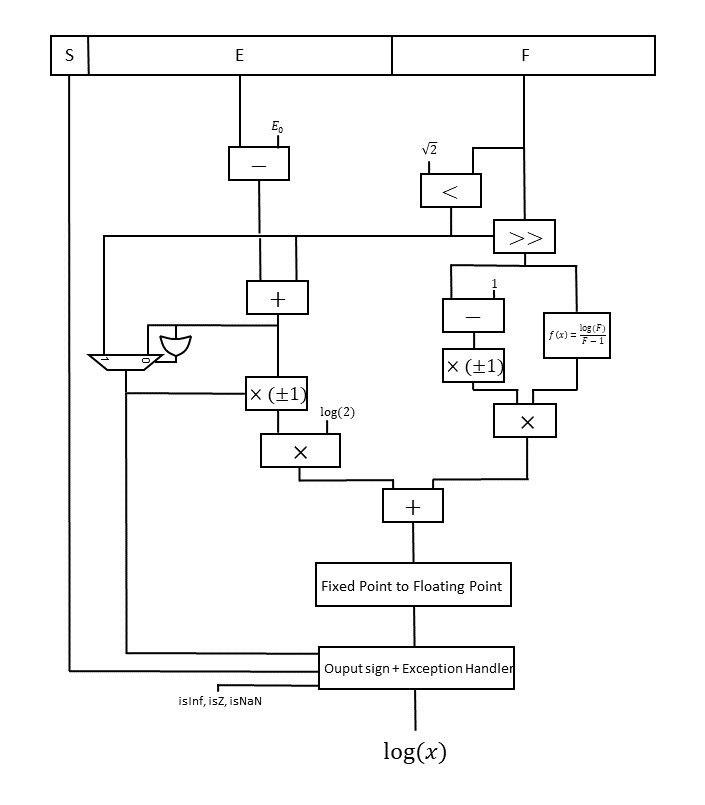
\includegraphics[width=0.7\textwidth]{images/block_diagram.jpg}
    \caption{Block design of the implemented algorithm}
\end{figure}
\newline
Some considerations:
\begin{itemize}
\item The function $f(x)=\dfrac{log(F)}{F-1}$ is implemented through a simple LUT with 8 input bits and 12 output bits.
\item The conversion from Fixed Point format to Bfloat16 is made with a “mask”.
\item The sign of the result is the sign of $(E-E_{0})$ (its MSB) when $(E-E_{0})\neq0$; otherwise it is given by the comparison between $F$ and $\sqrt{2}$.
\item Overflow and Underflow conditions are never met because the non-infinite output range goes from $[-92.0; +88.5]$ and the smallest ouput is $3.9e^{-3}$ (in modulus) so both the largest and smallest possible outputs are representable in Bfloat16 format.
\end{itemize}
    

\chapter{TestBench and Simulation}
Before instantiating the module in lampFPU\_top, a simulation was mandatory in order to check all possible errors and bugs.
\\It was decided to simulate the module on Vivado with an ad hoc testbench, so to fix in first approximation the main problems of the algorithm. To test the precision, a simulation with all of the acceptable inputs was executed (the full range from $S=0$  $E=0x00$  $F=0x00$ to $S=0$  $E=0xFF$  $F=0x7F$, 32768 values), the results were dumped on a csv file and parsed by means of a MATLAB script.
\\In the following figures, an error histogram is plotted, and the average and percentage errors are computed.
This script takes into account all the possible special cases in input, i.e. SNan, QNan.
The errors are more significant with respect to the simulations based on the DPI, because MATLAB is much more precise.
\begin{figure}[ht]
  \centering
    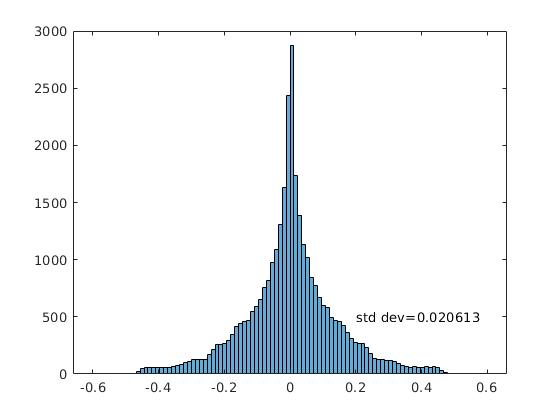
\includegraphics[width=0.7\textwidth]{images/hist.jpg}
    \caption{Histogram of the error.}
\end{figure}
    
\begin{figure}[ht]
  \centering
    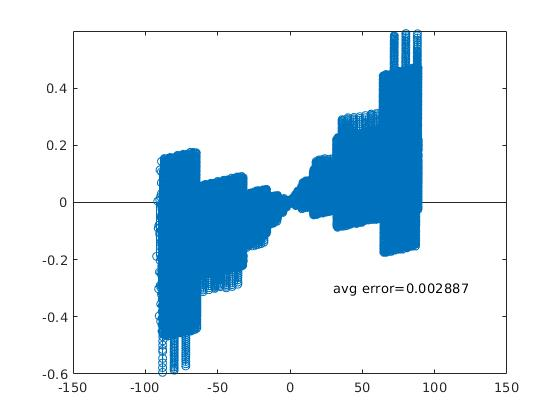
\includegraphics[width=0.7\textwidth]{images/avg_err.jpg}
    \caption{Committed error.}
\end{figure}

\begin{figure}[]
  \centering
    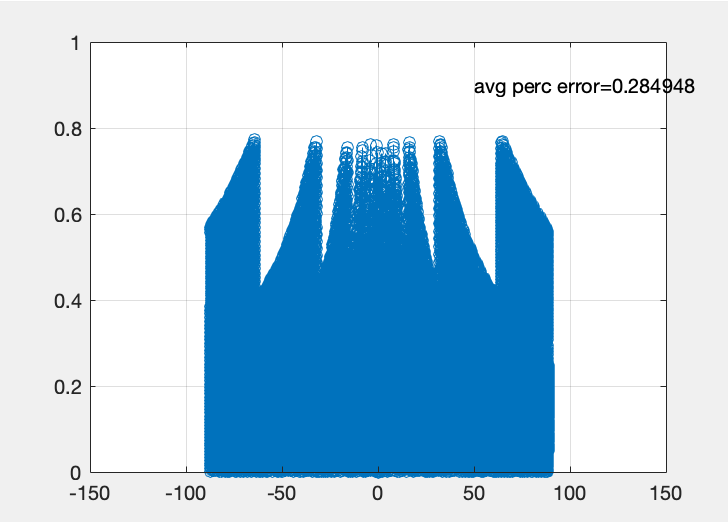
\includegraphics[width=0.7\textwidth]{images/avg_perc_err.png}
    \caption{Percentage error.}
\end{figure}
\chapter{Integration}
The aim of the project was to implement the natural logarithm module inside an already existing Floating Point Unit (FPU) provided by  Andrea Galimberti and Davide Zoni 
\footnote{\href{https://gitlab.com/davide.zoni/bfloat_fpu_systemverilog} {LAMP - BFloat16FPU} }

The signals used in the module are:

\begin{table}[htbp]
\begin{tabular}{|r|r|} 
\hline
\textbf{INPUT:}  & \textbf{COMMENT:}                          \\ 
\hline
clk              & clock signal                              \\ 
\hline
rst              & reset signal                              \\ 
\hline
doLog\_i         & activates the module                      \\ 
\hline
s\_op\_i         & sign of the input operand                 \\ 
\hline
extE\_op1\_i     & extended exponent of the input operand    \\ 
\hline
extF\_op1\_i     & extended fractional of the input operand  \\ 
\hline
isZ\_op\_i       & flag: true if input is zero               \\ 
\hline
isInf\_op\_i     & flag: true if input is infinite           \\ 
\hline
isSNAN\_op\_i    & flag: true if input is SNaN               \\ 
\hline
isQNAN\_op\_i    & flag: true if input is QNaN               \\ 
\hline
\hline
\textbf{OUTPUT:} &    \textbf{COMMENT:}                                       \\ 
\hline
s\_res\_o        & sign of the output                        \\ 
\hline
e\_res\_o        & exponent of the output                    \\ 
\hline
f\_res\_o        & fractional of the output                  \\ 
\hline
valid\_o         & asserted to 1 when the result is ready    \\ 
\hline
isOverflow\_o    & asserted to 1 when an overflow on the output is detected                   \\ 
\hline
ifUnderflow\_o   & asserted to 1 when an underflow on the output is detected                                                     \\ 
\hline
isToRound        & 1 if the output must be rounded           \\
\hline
\end{tabular}
\end{table}

The integration part consisted in the connection of the submodule to the top module, and the adding of the new state into the Finite State Machine logic.\\
Also the Package was modified, with the addition of the folllowing functions:\\
\colorbox{mygray}{\lstinline!LUT_log, FUNC_fix2float_log, FUNC_calcInfNanResLog! }
\\The first is a 8 bit look-up table used to calculate $\frac{log(F)}{F-1}$ \footnote{See Chapter 1 for more details};
\\The second is a function used to transform a fixed point number into a $BFloat_{16}$ SEF notation;
\\The last one is a function used to raise the correct output basing on the input flags. 

\bigskip
\section{Performances}

The whole algorithm performs within 6 clock cycles while from the $doLog\_i$ assertion to the raise of $isResultValid\_o$ register happens after just 3 clock cycles.

The algorithm had to be divided into a finite state machine with two states, because the multiplication operation between internal registers was too slow to perform within one clock cycle and so caused the presence of a negative slack.

\begin{table}[htbp]
\centering
\begin{tabular}{lll}
              & \textbf{W\textbackslash{}O LOG} & \textbf{W\textbackslash{} LOG}  \\
\textbf{LUT}  & 1065 (1.68\%)          & 1302 (2.05\%)             \\
\textbf{FF}   & 376 (0.3\%)			   & 399 (0.31\%)               \\
\textbf{DSP}  & 2 (0.83\%)             & 4 (1.67\%)             \\
\textbf{IO}   & 91 (43.33\%)           & 91 (43.33\%)           \\
\textbf{BUFG} & 1 (3.13\%)             & 1 (3.13\%)             \\
\textbf{WNS}  & 0.448ns                & 0.218ns                 
\end{tabular}
\end{table}


\begin{figure}[h]
  \centering
    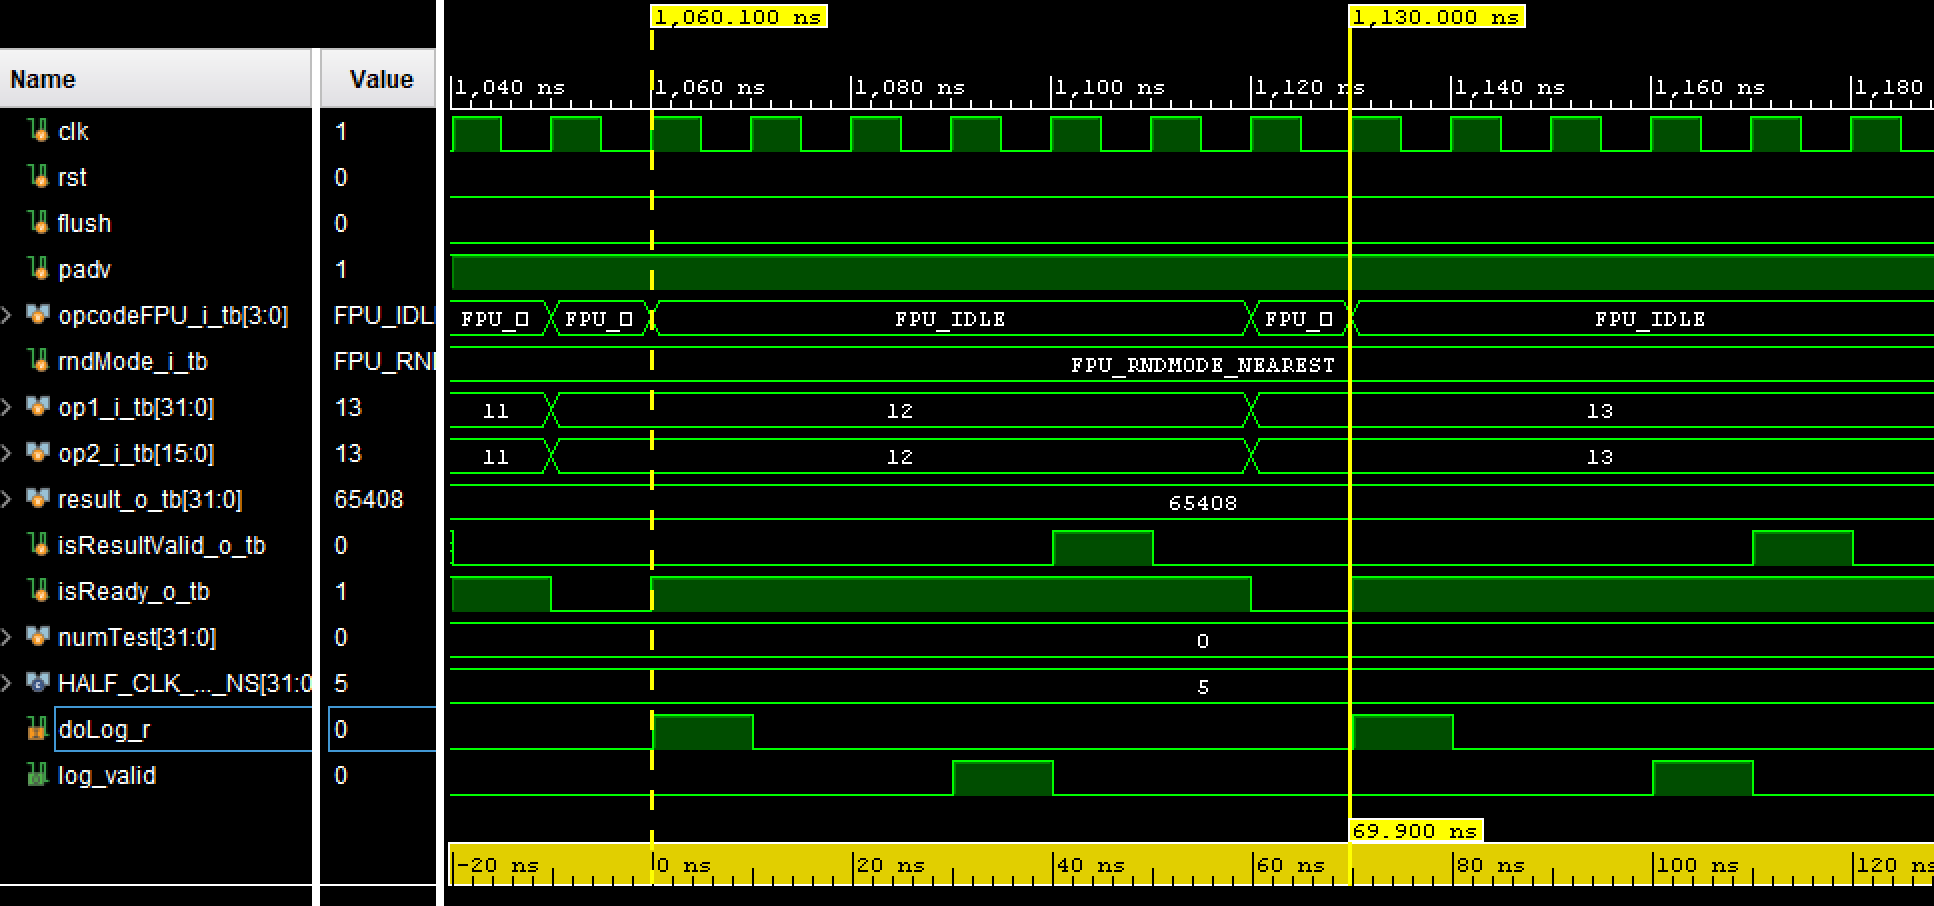
\includegraphics[width=0.8\textwidth]{images/waveforms.png}
    \caption{example waveforms of the Log module.}
\end{figure}

The simulation was done with the support of a Direct Programming Interface (DPI) that calculates the natural logarithm with the $math.h$ C library performed on a 32bit float value, and returns a 32bit floating point value, that then is transformed to bfloat16 by truncation. This translates into a discrepancy between some results calculated by the DPI and the ones calculated by the FPU-RTL module, with an error that is no bigger than 1LSB, due to the rounding to the next even performed on the FPU-RTL output.

\end{document}          
